%! TEX program = xelatex
% \documentclass[fontsize=12,draft]{scrartcl}
\documentclass[fontsize=12]{scrartcl}

\usepackage[sfdefault]{FiraSans}

\usepackage{setspace}
\onehalfspacing

\usepackage{lineno}
\linenumbers

\usepackage{pgfgantt}

\usepackage[skip=0pt]{parskip}
% \usepackage[libertine]{newtxmath}
% \usepackage[no-math]{fontspec}
% \usepackage{xltxtra}

\usepackage{polyglossia}
\setdefaultlanguage[variant=american]{english}
\setotherlanguage[babelshorthands]{german}

\usepackage{multirow}


\usepackage{placeins}

\usepackage{longtable}


\usepackage{url}

\usepackage[xetex,left=1.0cm,right=1cm,top=1.5cm,bottom=2cm]{geometry}

\usepackage{fixme}
\fxsetup{
    status=draft,
    author=,
    %layout=inline,
    theme=color,
    %layout=color,
    %targetlayout=color
}

\usepackage{graphicx}

\usepackage{amsmath}
\usepackage{natbib}
\usepackage{lineno,hyperref}
\usepackage{nicefrac}
\usepackage{soul}
\usepackage[colorinlistoftodos]{todonotes}
\newcommand{\hlfix}[2]{\texthl{#1}\todo{#2}}
\newcommand{\td}[1]{\todo[inline]{#1}}

\usepackage{xcolor}
\newcommand{\rr}[0]{{\color{red}{REVISE}}}

\usepackage{longtable}

\usepackage{fontawesome}

\usepackage{minted}

\begin{document}
\section{Summary}

More information, and introductions to the concepts of the \textbf{data tree}
and corresponding \textbf{metadata} can be found at the project source
repository:

\url{https://github.com/geophysics-ubonn/ubg_data_toolbox}

\subsection{The DataTools in the Jupyter terminal}

The following commands can be run in all standard terminal. We recommend to use
a Jupyter Terminal.

Note that the Python package \textsl{ubg\_data\_toolbox} must be installed. This
can be done by executing:

\begin{minted}{bash}
pip install ubg_data_toolbox
\end{minted}

You can also install the toolbox from within a Jupyter Notebook cell by
executing:

\begin{minted}{bash}
!pip install ubg_data_toolbox
\end{minted}

% \begin{itemize}
%     \item On first login into the Jupyer hub:
%         \begin{minted}{bash}
%                 conda init
%         \end{minted}
%     \item For each terminal session:
%         \begin{minted}{bash}
%                 conda activate code-data-tools
%         \end{minted}
% \end{itemize}

\subsection{The Commands}

The following commands are used to manage \textbf{data trees}:

\begin{itemize}
    \item Check a single measurement (\textbf{m\_*}) directory:
        \begin{minted}{bash}
                dm_m_check_dir
        \end{minted}
    \item Check a complete data directory (\textbf{dm\_*}) directory:
        \begin{minted}{bash}
                dm_check_dirtree
        \end{minted}
	\item Add data (file(s) or directory) to a data tree, interactively:
        \begin{minted}{bash}
            dm_add
        \end{minted}
    \item Initialise a new \textsl{metadata.ini} based on the directory structure:
        \begin{minted}{bash}
            dm_init_metadata
        \end{minted}
    \item List all measurement directories
        \begin{minted}{bash}
            dm_list_measurements
        \end{minted}
\end{itemize}

Usually command line options can be queried by appending "-h" to the command.
Example:
\begin{minted}{bash}
$ dm_add -h
usage: dm_add [-h] -t TREE -i INPUT [INPUT ...]

Add one measurement to a given data directory structure

options:
  -h, --help            show this help message and exit
  -t TREE, --tree TREE  Path of data tree (should start with: dr_
  -i INPUT [INPUT ...], --input INPUT [INPUT ...]
                        Path to measurement (data/directory/directory tree)
\end{minted}

\subsection{Procedures}

\begin{itemize}
	\item In absence of a data tree, use \textbf{dm\_add} to add measurements
		to a newly created directory structure
	\item For additional measurements, it usually is also convenient to keep on
		using \textbf{dm\_add}. However, you can also use the following procedure:
		\begin{itemize}
			\item Create the \textbf{m\_*} in the correct place BEFORE creating the
				\textsl{metadata.ini} file.
			\item THEN, use \textbf{dm\_init\_metadata} to initiate the
				\textsl{metadata.ini} file from the directory structure. Note
				that there may be missing, but required, metadata entries that
				can not be extracted automatically from the directory tree.
		\end{itemize}
	\item Check the directory tree with \textbf{dm\_check\_dirtree} and fix any
		reported issues
\end{itemize}

\section{Directory Structure}

The directory structure is defined as follows. Each directory must start with a
prefix, followed by an underscore, followed by a name/value. For example, the
top directory could be called: \textbf{dr\_datatree}.

Note that some levels are optional (indicated by additional arrows in the
figure below).

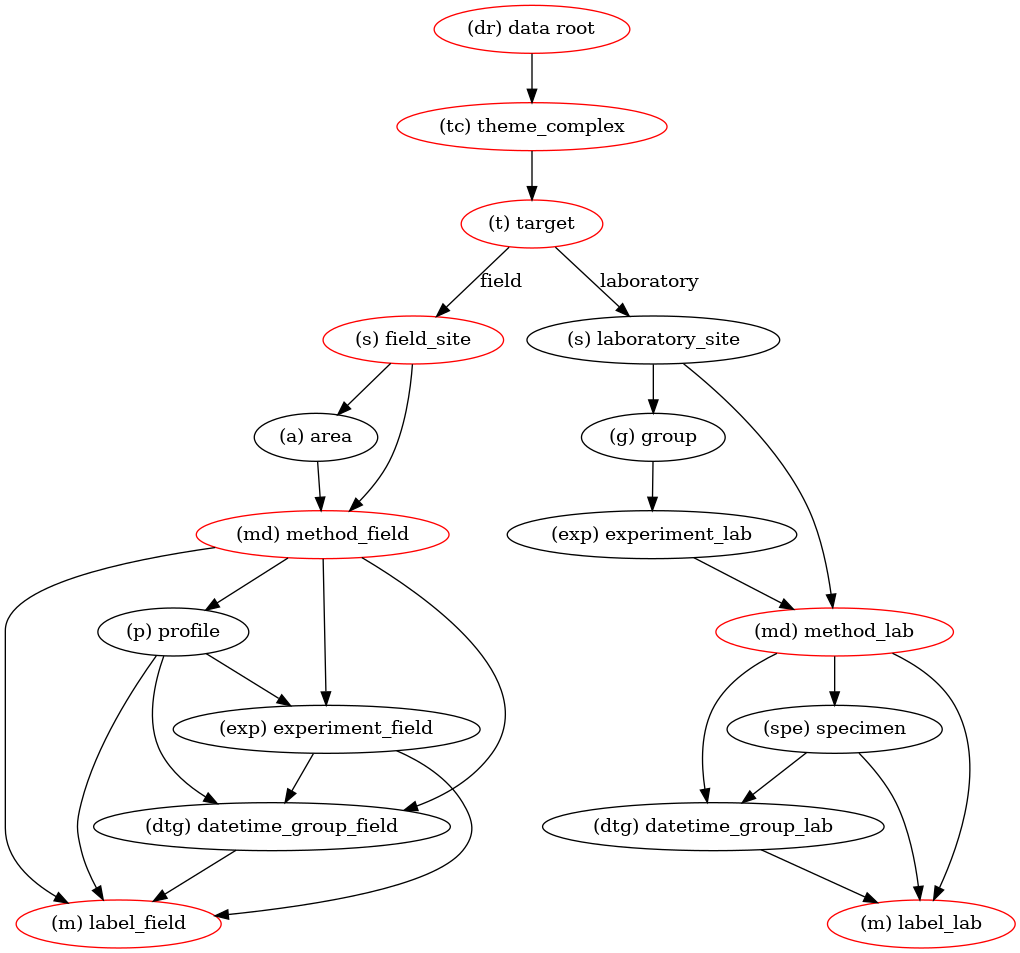
\includegraphics[width=\textwidth]{dirtree.png}

An example a directory tree (with only one measurement) is:

\begin{minted}{bash}
  └── dr_datatree/
    └── tc_hydrogeophysics
        └── t_field
            └── s_Spiekeroog
                └── a_North
                    └── md_ERT
                        └── p_p_01_nor
                            └── m_01_p1_nor
                                ├── metadata.ini
                                └── RawData
                                    └── data.dat
\end{minted}

\clearpage
\section{Metadata}

Metadata is collected in \textsl{metadata.ini} files that reside in the
individual measurement (m\_)-directories.

An example \textsl{metadata.ini} file could look like:

\begin{minted}{ini}
[general]
label = 20240610_ert_p1_nor
person_responsible = Maximilian Weigand
person_email = mw@domain.com
theme_complex = Hydrogeophysics
datetime_start = 20240610_1200
description = A small test measurement
    Note that some entries are multi-line capable!
survey_type = field
method = ERT
completed = yes

[field]
site = Spiekeroog
area = north
profile = p_01

[geoelectrics]
profile_direction = normal
\end{minted}

You can add arbitrary \textsl{[sections]} and key=value pairs. However, the
following set of metadata entries is pre-defined, with some of the
\textbf{required}:
\newpage
{\footnotesize
\begin{longtable}{c|c|c|c|c|p{6cm}}
key & multi-line & required field & required lab &Doublin Core & description\\
\hline
section: [general]\\
\hline
label & \faTimes & True & True &  & Label of the individual measurement, This is the identifier for a given measurement at a given profile. Usually we construct the label using three parts: datetime, running number, one or two important keywords. Example: 20240516\_01\_p1\_nor \\
person\_responsible & \faTimes & True & True & creator & The person that is responsible for this data set. This must not necessarily be the person that conducted the measurement. \\
person\_email & \faTimes & True & True &  & Email address of the person now maintaining this data set. \\
attending\_persons & \faTimes & False & False & contributor & All persons that were involved during the measurement. Optional: Add email addresses in parentheses, e.g. Maximilian Weigand (mweigand@geo.uni-bonn.de) \\
theme\_complex & \faTimes & True & True & subject & Theme complex that the measurement falls under. This is the most general category for a given measurement \\
project & \faTimes & False & False & part of title & ? \\
datetime\_start & \faTimes & True & True & date & Starting datetime of the measurement/measurements. Use date format YYYYmmdd\_HHMM\_s . YYYY: Year (e.g., 2004), mm: Month, dd: Day of month, HH: hour (1-24), MM: Minute (1-60), SS: Second Leave unknown parts out (e.g., seconds) \\
datetime\_end & \faTimes & False & False & date & Ending datetime of the measurement/measurements \\
description & \faCheck & True & True & description & Description (should be short, comprehensive, and with links to detailed documentation) \\
survey\_type & \faTimes & True & True &  & Field or laboratory measurements? Allowed values: field, laboratory \\
method & \faTimes & True & True & False & Which method(s) were used? (e.g.: ERT, SP, GPS, GPR) \\
experiment & \faTimes & False & False &  & Label for the experiment that a measurement is assigned to \\
description\_exp & \faCheck & False & False &  & Description (should be short, comprehensive, and link to detailed documentation) \\
restrictions & \faCheck & False & False & license & State any licensing restriction of the data set. Especially, note down any copyright owned by a party that is not the Department of Geophysics, Uni Bonn \\
completed & \faTimes & True & True &  & States if the measurement series is finished or still ongoing. Possible values: yes, no \\
keywords & \faTimes & False & False & subject & Keywords, separated by comma. \\
related\_dois & \faCheck & False & False & references &  \\
missing & \faCheck & False & False &  & ? \\
problems & \faCheck & False & False &  & Known restrictions/problems of the dataset (entries should be time stamped, multi-line entries required) \\
signed\_off\_by & \faCheck & False & False &  & ? \\
analysis\_links & \faCheck & False & False &  & ? \\
dt\_group & \faTimes & False & False &  & Datetime group -- Used to group measurements, e.g. into days or years \\
\hline
section: [field]\\
\hline
survey\_start & \faTimes & False & False &  & Starting datetime of survey. Intended for the field data tree. Format: yyyymmdd hh:mm:ss \\
survey\_end & \faTimes & False & False &  & Ending datetime of survey. Intended for the field data tree. Format: yyyymmdd hh:mm:ss (same as survey\_start) \\
site & \faTimes & True & False &  & The general area of the measurement, e.g. a town name. This is further clarified in the metadata entries "area", "profile", "coordinates" \\
area & \faTimes & True & False &  & A more localized specification of the measurement area, e.g., an identifier of a certain field or street \\
profile & \faTimes & True & False &  & The profile that was measured on. One common naming scheme consistent of the character "p",a running number, and a signifying key word. Example: p\_01\_nor \\
coordinates & \faCheck & False & False &  & Coordinates of representative location(s) (i.e., starting point of measurement profile). One coordinate per line The use of WGS84 coordinates is preferred (EPSG 4326). Please state the use of other coordinate systems in the metadata entry "coordinates\_desc". Coordinates should be included in decimal notation, with a least 6 decimal digits (ca. 5-12cm precision). https://wiki.openstreetmap.org/wiki/Precision\_of\_coordinates \\
coordinates\_desc & \faCheck & False & False &  & Description of coordinates. State used representation (e.g., WGS84 or UTM) here. Do not forget the UTM zone \\
\hline
section: [geoelectrics]\\
\hline
spacing & \faTimes & False & False &  & Electrode spacing \\
profile\_direction & \faTimes & True & False &  & Profile direction. Allowed values: normal, reciprocal \\
electrode\_positions & \faCheck & True & False &  & Electrode positions (x,y,z) \\
\hline
section: [laboratory]\\
\hline
site & \faTimes & False & True &  & Laboratory measurement site \\
group & \faTimes & False & False &  & High-level group of experiments \\
experiment\_start & \faTimes & False & False &  & Starting datetime of experiment. Intended for the laboratory data tree. Format: yyyymmdd hh:mm:ss \\
experiment\_end & \faTimes & False & False &  & Ending datetime of experiment. Intended for the laboratory data tree. Format: yyyymmdd hh:mm:ss (same as experiment\_start) \\
specimen & \faTimes & False & False &  & Sample material, e.g. sandstone; used mainly for laboratory measurement metadata. \\
permeability & \faTimes & False & False &  & Permeability of sample material \\
porosity & \faTimes & False & False &  & Porosity of sample material \\
\hline
section: [device]\\
\hline
device & \faTimes & False & False &  & Used measurement instrument. \\
device\_serial & \faTimes & False & False &  & Serial number of instrument, required if several devices of one type exist (e.g. the DT80) \\
programming & \faTimes & False & False &  & Optional file path to a script/file containing the programming (script) used for the measurements(s) \\
\end{longtable}
}
\end{document}
